%% LyX 2.1.2.1 created this file.  For more info, see http://www.lyx.org/.
%% Do not edit unless you really know what you are doing.
\documentclass[10pt,english]{beamer}
\usepackage[T1]{fontenc}
\usepackage[latin9]{inputenc}
\usepackage{amsthm}
\usepackage{amsmath}
\usepackage{amssymb}
\usepackage{tikz}

\DeclareMathOperator{\E}{\mathbb{E}}
\DeclareMathOperator*{\argmin}{arg\,min}

\makeatletter
%%%%%%%%%%%%%%%%%%%%%%%%%%%%%% Textclass specific LaTeX commands.
 % this default might be overridden by plain title style
 \newcommand\makebeamertitle{\frame{\maketitle}}%
 % (ERT) argument for the TOC
 \AtBeginDocument{%
   \let\origtableofcontents=\tableofcontents
   \def\tableofcontents{\@ifnextchar[{\origtableofcontents}{\gobbletableofcontents}}
   \def\gobbletableofcontents#1{\origtableofcontents}
 }

%%%%%%%%%%%%%%%%%%%%%%%%%%%%%% User specified LaTeX commands.
\usepackage{listings}
\usetheme{Warsaw}
% or ...
%\usetheme{Antibes}	% tree outline, neat
%\usetheme{JuanLesPins}	% like Antibes, with shading
%\usetheme{Bergen}	% outline on side
%\usetheme{Luebeck}	% like Warsaw, square sides
%\usetheme{Berkeley}	% interesting left bar outline
%\usetheme{Madrid}	% clean, nice.  7/12 page numbers
%\usetheme{Berlin}	% dots show slide number
%\usetheme{Malmoe}	% OK, plain, unshaded
%\usetheme{Boadilla}	% nice, white bg, no top bar
%\usetheme{Marburg}	% nice, outline on right
%\usetheme{boxes}	% ???
%\usetheme{Montpellier}	% tree outline on top, plainish white
%\usetheme{Copenhagen}	% like Warsaw
%\usetheme{PaloAlto}	% looks good
%\usetheme{Darmstadt}	% like Warsaw with circle outline
%\usetheme{Pittsburgh}
%\usetheme{default}
%\usetheme{Rochester}	% like boxy, unshaded warsaw
%\usetheme{Dresden}	% circle outline on top
%\usetheme{Singapore}	% purple gradient top
%\usetheme{Frankfurt}	% like Warsaw with circle outline on top
%\usetheme{Szeged}
%\usetheme{Goettingen}	% light purple right bar outline
%\usetheme{Warsaw}
%\usetheme{Hannover}	% like Goett with bar on left
%\usetheme{compatibility}
%\usetheme{Ilmenau}

\setbeamercovered{transparent}
% or whatever (possibly just delete it)

%\usecolortheme{seahorse}
%\usecolortheme{rose}

% seems to fix typewriter font in outline header:
\usepackage{ae,aecompl}

\makeatother

\usepackage{babel}

\title{Performance Comparisons of the K-Means Algorithm}
\author{Mark A. Ward}
\institute{Center for Data Science, NYU}
\begin{document}


\pgfdeclareimage[height=0.5cm]{institution-logo}{institution-logo-filenameO}

\logo{\pgfuseimage{institution-logo}}

% RPD:  can't get this to work on any template.  not present in Warsaw any way, it seems

% hmm, problem seems to be that it isn't copied to the tmp dir, probably becuase it doesn't have the

% filename extension (which is tacked on by pgf it seems)

%\AtBeginSection[]{
\begin{frame}
\titlepage
\end{frame}
\AtBeginSection[]{

  \frame<beamer>{ 

    \frametitle{Outline}   

    \tableofcontents[currentsection,currentsubsection] 
%    \tableofcontents[currentsection] 

  }

}
%\beamerdefaultoverlayspecification{<+->}
\begin{frame}
     \frametitle{Outline}   
    \tableofcontents[currentsection,currentsubsection,sectionstyle = show,subsectionstyle = show] 
\end{frame}

\section{Introduction}
\subsection{The K-Means Algorithm}
\begin{frame}
\frametitle{\insertsubsection}
\begin{itemize}
	\item Algorithm that aims to partition $n$ observations into $k$ clusters where each observation belongs to the cluster nearest mean or centroid
	\item Vector quantization in signal processing
	\item Cluster analysis in data mining, how do you choose $k$?
	\item Feature learning in semi-supervised or unsupervised learning
	\item Clustering is NP-hard, but k-means is a heuristic that converges quickly to a local optimum
	\item Typical running time $O(nkdi)$, repeat for $T$ trials
	\item For $n$ points in $[0,1]^d$ with independent gaussian perturbations with $0$ mean and $\sigma^2$ variance, upper bound expected running time by $O(n^{34} k^{34} d^8 \text{log}^4(n) / \sigma^6)$. [Arthur 2009]
\end{itemize}
\end{frame}

\begin{frame}{\insertsubsection}
\begin{figure}
\includegraphics[keepaspectratio=true, width=4.0in]{algo.png}
\end{figure}
\end{frame}

%%%%%%%%%%%%%%%%%%%%%
\subsection{Examples}

\begin{frame}{\insertsubsection}
\begin{figure}
\includegraphics[keepaspectratio=true, width=4.0in]{data_blobs.png}
\end{figure}
\end{frame}
\begin{frame}{\insertsubsection}
\begin{figure}
\includegraphics[keepaspectratio=true, width=4.0in]{center_initialization.png}
\end{figure}
\end{frame}

\begin{frame}{\insertsubsection}
\begin{figure}
\includegraphics[keepaspectratio=true, width=4.0in]{kmeans_iter_1a.png}
\end{figure}
\end{frame}
\begin{frame}{\insertsubsection}
\begin{figure}
\includegraphics[keepaspectratio=true, width=4.0in]{kmeans_iter_1b.png}
\end{figure}
\end{frame}

\begin{frame}{\insertsubsection}
\begin{figure}
\includegraphics[keepaspectratio=true, width=4.0in]{kmeans_iter_2a.png}
\end{figure}
\end{frame}
\begin{frame}{\insertsubsection}
\begin{figure}
\includegraphics[keepaspectratio=true, width=4.0in]{kmeans_iter_2b.png}
\end{figure}
\end{frame}

\begin{frame}{\insertsubsection}
\begin{figure}
\includegraphics[keepaspectratio=true, width=4.0in]{kmeans_iter_3a.png}
\end{figure}
\end{frame}
\begin{frame}{\insertsubsection}
\begin{figure}
\includegraphics[keepaspectratio=true, width=4.0in]{kmeans_iter_3b.png}
\end{figure}
\end{frame}

\begin{frame}{\insertsubsection}
\begin{figure}
\includegraphics[keepaspectratio=true, width=4.0in]{kmeans_iter_4a.png}
\end{figure}
\end{frame}
\begin{frame}{\insertsubsection}
\begin{figure}
\includegraphics[keepaspectratio=true, width=4.0in]{kmeans_iter_4b.png}
\end{figure}
\end{frame}

\begin{frame}{\insertsubsection}
\begin{figure}
\includegraphics[keepaspectratio=true, width=4.0in]{kmeans_iter_5a.png}
\end{figure}
\end{frame}
\begin{frame}{\insertsubsection}
\begin{figure}
\includegraphics[keepaspectratio=true, width=4.0in]{kmeans_iter_5b.png}
\end{figure}
\end{frame}

\begin{frame}{\insertsubsection}
\begin{figure}
\includegraphics[keepaspectratio=true, width=4.0in]{kmeans_iter_6a.png}
\end{figure}
\end{frame}
\begin{frame}{\insertsubsection}
\begin{figure}
\includegraphics[keepaspectratio=true, width=4.0in]{kmeans_iter_6b.png}
\end{figure}
\end{frame}

%%%%%%%%%%%%%%%%%%%%%

\begin{frame}{\insertsubsection}
\begin{center}
	229,931 colors
\end{center}
\begin{figure}
	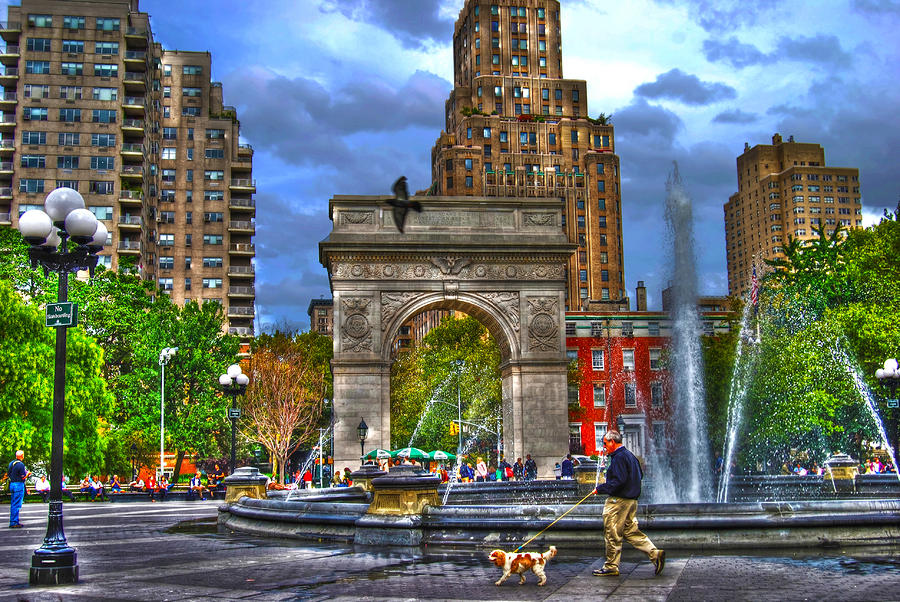
\includegraphics[keepaspectratio=true, width=3.9in]{wsqpark.png}
\end{figure}
\end{frame}

\begin{frame}{\insertsubsection}
\begin{center}
	256 colors
\end{center}\begin{figure}
	\includegraphics[keepaspectratio=true, width=3.9in]{wsqpark256.png}
\end{figure}
\end{frame}

\begin{frame}{\insertsubsection}
\begin{center}
	128 colors
\end{center}\begin{figure}
	\includegraphics[keepaspectratio=true, width=3.9in]{wsqpark128.png}
\end{figure}
\end{frame}

\begin{frame}{\insertsubsection}
\begin{center}
	64 colors
\end{center}
\begin{figure}
	\includegraphics[keepaspectratio=true, width=3.9in]{wsqpark64.png}
\end{figure}
\end{frame}

\begin{frame}{\insertsubsection}
\begin{center}
	32 colors
\end{center}
\begin{figure}
	\includegraphics[keepaspectratio=true, width=3.9in]{wsqpark32.png}
\end{figure}
\end{frame}

\begin{frame}{\insertsubsection}
\begin{center}
	16 colors
\end{center}
\begin{figure}
	\includegraphics[keepaspectratio=true, width=3.9in]{wsqpark16.png}
\end{figure}
\end{frame}

\begin{frame}{\insertsubsection}
\begin{center}
	10 colors
\end{center}
\begin{figure}
	\includegraphics[keepaspectratio=true, width=3.9in]{wsqpark10.png}
\end{figure}
\end{frame}

\begin{frame}{\insertsubsection}
\begin{center}
	5 colors
\end{center}
\begin{figure}
	\includegraphics[keepaspectratio=true, width=3.9in]{wsqpark5.png}
\end{figure}
\end{frame}

\begin{frame}{\insertsubsection}
\begin{center}
	3 colors
\end{center}
\begin{figure}
	\includegraphics[keepaspectratio=true, width=3.9in]{wsqpark3.png}
\end{figure}
\end{frame}

\begin{frame}{\insertsubsection}
\begin{center}
	2 colors
\end{center}
\begin{figure}
	\includegraphics[keepaspectratio=true, width=3.9in]{wsqpark2.png}
\end{figure}
\end{frame}

%%%%%%%%%%%%%%%%%%%%%%%%

\section{Parallel K-Means}
\subsection{MPI Communication Overview}

\begin{frame}{\insertsubsection}
\begin{center}
	\begin{tikzpicture}
		\node[anchor=south west,inner sep=0] (image) at (0,0) {\includegraphics[keepaspectratio=true, width=4.0in]{algo.png}};
	\end{tikzpicture}
\end{center}
\end{frame}

\begin{frame}{\insertsubsection}
\begin{center}
	\begin{tikzpicture}
		\node[anchor=south west,inner sep=0] (image) at (0,0) {\includegraphics[keepaspectratio=true, width=4.0in]{algo.png}};
		\node[align=center,red,font={\bfseries}] at (2.05,5.95) {Distribute objects};
	\end{tikzpicture}
\end{center}
\end{frame}

\begin{frame}{\insertsubsection}
\begin{center}
	\begin{tikzpicture}
		\node[anchor=south west,inner sep=0] (image) at (0,0) {\includegraphics[keepaspectratio=true, width=4.0in]{algo.png}};
		\node[align=center,red,font={\bfseries}] at (2.05,5.95) {Distribute objects};
		\node[align=center,red,font={\bfseries}] at (2.05,5.05) {BCast Centers};
	\end{tikzpicture}
\end{center}
\end{frame}

\begin{frame}{\insertsubsection}
\begin{center}
	\begin{tikzpicture}
		\node[anchor=south west,inner sep=0] (image) at (0,0) {\includegraphics[keepaspectratio=true, width=4.0in]{algo.png}};
		\node[align=center,red,font={\bfseries}] at (2.05,5.95) {Distribute objects};
		\node[align=center,red,font={\bfseries}] at (2.05,5.05) {BCast Centers};
		\node[align=center,red,font={\bfseries}] at (2.05,2.88) {AllReduce x2};
	\end{tikzpicture}
\end{center}
\end{frame}

\begin{frame}{\insertsubsection}
\begin{center}
	\begin{tikzpicture}
		\node[anchor=south west,inner sep=0] (image) at (0,0) {\includegraphics[keepaspectratio=true, width=4.0in]{algo.png}};
		\node[align=center,red,font={\bfseries}] at (2.05,5.95) {Distribute objects};
		\node[align=center,red,font={\bfseries}] at (2.05,5.05) {BCast Centers};
		\node[align=center,red,font={\bfseries}] at (2.05,2.88) {AllReduce x2};
		\node[align=center,red,font={\bfseries}] at (2.05,1.88) {AllReduce x2};
	\end{tikzpicture}
\end{center}
\end{frame}

\subsection{Initialization}

\begin{frame}{\insertsubsection}
\begin{figure}
	\includegraphics[keepaspectratio=true, width=3.9in]{init0.png}
\end{figure}
\end{frame}

\begin{frame}{\insertsubsection}
\begin{figure}
	\includegraphics[keepaspectratio=true, width=3.9in]{init1.png}
\end{figure}
\end{frame}

\begin{frame}{\insertsubsection}
\begin{figure}
	\includegraphics[keepaspectratio=true, width=3.9in]{init2.png}
\end{figure}
\end{frame}

\begin{frame}{\insertsubsection}
\begin{figure}
	\includegraphics[keepaspectratio=true, width=3.9in]{init3.png}
\end{figure}
\end{frame}

\begin{frame}{\insertsubsection}
\begin{figure}
	\includegraphics[keepaspectratio=true, width=3.9in]{init4.png}
\end{figure}
\end{frame}

\begin{frame}{\insertsubsection}
\begin{figure}
	\includegraphics[keepaspectratio=true, width=3.9in]{init5.png}
\end{figure}
\end{frame}

\begin{frame}{\insertsubsection}
\begin{figure}
	\includegraphics[keepaspectratio=true, width=3.9in]{init6.png}
\end{figure}
\end{frame}

\begin{frame}{\insertsubsection}
\begin{figure}
	\includegraphics[keepaspectratio=true, width=3.9in]{init7.png}
\end{figure}
\end{frame}

\begin{frame}{\insertsubsection}
\begin{figure}
	\includegraphics[keepaspectratio=true, width=3.9in]{init8.png}
\end{figure}
\end{frame}

%%%%%%%%%%%%%%%%%%%%%%%%

\section{Concluding Remarks}
\begin{frame}
   \frametitle{\insertsubsection}
  \begin{itemize}
  \item THE END
  \end{itemize}
\end{frame}

\begin{frame}[allowframebreaks]
  \frametitle<presentation>{Further Reading}    
  \begin{thebibliography}{10}    
\tiny
  \beamertemplatearticlebibitems
  \bibitem{Arthur2009}
Arthur, David and Manthey, Bodo and Roglin, H
\newblock{\em k-Means has polynomial smoothed complexity}
\newblock Foundations of Computer Science, 2009. FOCS'09. 50th Annual IEEE Symposium on. (2009) 405-414

  \beamertemplatearticlebibitems
  \bibitem{macqueen1967}
MacQueen, James and others
\newblock{\em Some methods for classification and analysis of multivariate observations}
\newblock Proceedings of the fifth Berkeley symposium on mathematical statistics and probability. (1967) 281-297


\end{thebibliography}
\end{frame}   
\end{document}


